\documentclass[11pt]{article}
\usepackage{tikz}
\usetikzlibrary{positioning,fit,backgrounds}
\usepackage[normalem]{ulem}
\usepackage{cs1200}

\begin{document}

% To include a problems set header, use the psHeader command
\psHeader{6}{Thu Nov. 12, 2026 (11:59pm)}

Please see the syllabus for the full collaboration and generative AI policy, as well as information on grading, late days, and revisions.

All sources of ideas, including (but not restricted to) any collaborators, AI tools, people outside of the course, websites, ARC tutors, and textbooks other than Hesterberg--Vadhan must be listed on your submitted homework along with a brief description of how they influenced your work. You need not cite core course resources, which are lectures, the Hesterberg--Vadhan textbook, sections, SREs, problem sets and solutions sets from earlier in the semester. If you use any concepts, terminology, or problem-solving approaches not covered in the course material by that point in the semester, you must describe the source of that idea. If you credit an AI tool for a particular idea, then you should also provide a primary source that corroborates it. Github Copilot and similar tools should be turned off when working on programming assignments.

If you did not have any collaborators or external resources, please write 'none.' A problem set on the border between two letter grades cannot be rounded up if collaborators are not noted.

\vspace{1em}

\textbf{Your name: }

\textbf{Collaborators and External Resources: }

\textbf{No. of late days used on previous psets: }

\textbf{No. of late days used after including this pset: }

\vspace{1em}

The purpose of this problem set is to practice modeling problems using graphs, reinforce understanding of the matching algorithm we learned, practice the resolution algorithm and reductions to SAT, and think about ethical issues raised when modeling real-world problems for algorithmic solution.

\begin{enumerate}

 \item (Matching Algorithms)
 Another practical application of matching algorithms is planning logistics, like in the following example from (fictional) ridesharing service Lyber in (real) New York City's Times Square.  When a customer books a Lyber ride, the ride request is sent to a Lyber server and combined with others to create a schematic like the one drawn in the map below.

\begin{figure}[h]
    \centering
    \includegraphics[width=0.55\textwidth]{{Spring26/Problem Sets/ps7/ps7_diagram.png}}
    \label{fig:travel_time_graph}
\end{figure}

Given a schematic like this, Lyber's goal is to serve as many customers (labeled A--E in the map) as possible, by assigning each one to a driver (labeled 1--6 in the map). For simplicity, each customer and driver is at an intersection, and assume driving between adjacent streets (vertical segment) takes 30 seconds, and driving between adjacent avenues (horizontal segments) takes 1 minute. However, the one twist is that they want to make sure that \textit{no customer is waiting for longer than 2 minutes}.  They also do not want to assign a driver to more than one customer at once, since serving a single customer can take more than 2 minutes.

    \begin{enumerate}
    \item To perform the assignment, they reduce to \MaximumMatching\ in bipartite graphs.  Draw a bipartite graph corresponding to the drivers and customers in the map above.
    \item The Lyber app first prioritizes customers on Broadway, so they initially assign customer $A$ to driver 3 and customer $C$ to driver 5. Using the algorithm from class, find a \textit{maximum matching} in the bipartite matching graph you've drawn, starting from the initial matching of $A$ to 3 and $C$ to 5. Draw pictures showing the sequence of matchings and augmenting paths you find. (No need to break down the steps of the algorithm to find the augmenting paths.)    \end{enumerate}

\item (Resolution)
Use the algorithm \texttt{ResolutionInOrder} (Algorithm 18.2 from Section 18.1 in the textbook) to decide the satisfiability of the following formula, and if it is satisfiable, use the algorithm \texttt{ExtractAssignment} (Algorithm 18.4 in Section 18.2 of the textbook) to obtain a satisfying assignment. (Please make sure to follow both algorithms \textit{exactly}, including the order in which the clauses are processed. A correct final solution that does not show all of the intermediate steps of the algorithms will not receive full score. You may omit resolvents that are $1$ or duplicates of existing clauses.)
 
\[\varphi(x_0, x_1, x_2, x_3) = (x_0 \vee x_1) \wedge (\neg x_0 \vee x_2) \wedge (\neg x_1 \vee \neg x_2) \wedge (x_2 \vee x_3)\]

\item (Reductions to SAT) In Section 15.3 of the textbook, we saw an efficient algorithm to solve the Maximum Matching problem in Bipartite Graphs. A variant of Maximum Matching is Maximum 3-D Matching, where we are given not a graph $G=(V,E)$ but a ``3-uniform hypergraph'' $H=(V,E)$, where the {\em hyperedges} $e\in E$ now are {\em triples} of vertices.
Analogously to restricting to bipartite graphs, we restrict to {\em tripartite} hypergraphs where $V$ is the union of 3 disjoint sets $V_0\cup V_1 \cup V_2$ and every hyperedge $e\in E$ has exactly one vertex from each of $V_0,V_1,V_2$. For example, hyperedges may consist of
compatible patient-donor-timeslot triples (if there are only certain timeslots in which a patient and donor are available for a surgery),
or compatible surfer-surfboard-fins triples (if each surfer only likes to ride certain surfboards with certain fins installed).
Now the goal is to find a maximum-sized set $M\subseteq E$ such that every vertex $v\in V$ is contained in at most one edge of $M$.
Unfortunately, unlike matching in graphs, there is no polynomial-time algorithm known for Maximum 3-D Matching, even if we restrict to tripartite hypergraphs and even if we only want to find {\em complete matchings} --- ones that match every vertex in $V_0$ (i.e. we are looking for a matching of size $|M|=|V_0|$):
\compprob{3dCompleteMatching()}
{Three disjoint finite sets of vertices $V_0,V_1,V_2$ and a set $E$ of hyperedges  such that each $e\in E$ contains exactly one vertex from each of $V_0$, $V_1$, and $V_2$.}
{A set $M$ of hyperedges such that every vertex is in at most one hyperedge in $M$, and every vertex in $V_0$ is in some hyperedge in $M$ (if one exists).
}

\begin{figure}[h]
\centering
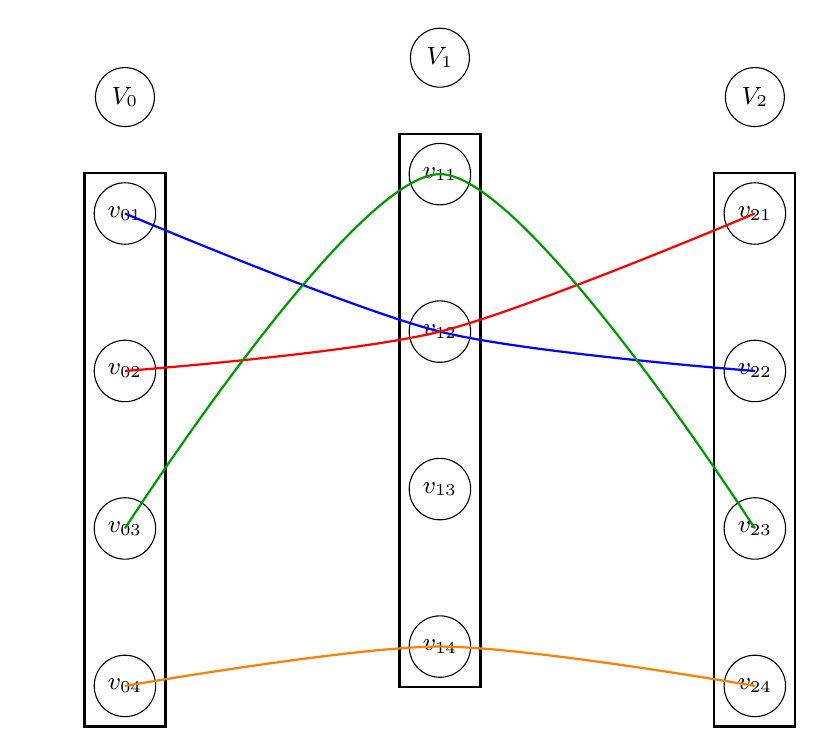
\begin{tikzpicture}[
  every node/.style={circle, draw, minimum size=7mm, font=\small},
  edge/.style={thick, bend left=15}
]

\node (v01) at (0,3) {$v_{01}$};
\node (v02) at (0,1) {$v_{02}$};
\node (v03) at (0,-1) {$v_{03}$};
\node (v04) at (0,-3) {$v_{04}$};

\node (v11) at (4,3.5) {$v_{11}$};
\node (v12) at (4,1.5) {$v_{12}$};
\node (v13) at (4,-0.5) {$v_{13}$};
\node (v14) at (4,-2.5) {$v_{14}$};

\node (v21) at (8,3) {$v_{21}$};
\node (v22) at (8,1) {$v_{22}$};
\node (v23) at (8,-1) {$v_{23}$};
\node (v24) at (8,-3) {$v_{24}$};

\node[above=0.7cm of v01] {$V_0$};
\node[above=0.7cm of v11] {$V_1$};
\node[above=0.7cm of v21] {$V_2$};

\begin{pgfonlayer}{background}
  \node[draw, thick, shape=rectangle, fit=(v01) (v02) (v03) (v04), label=left:{}] {};
  \node[draw, thick, shape=rectangle, fit=(v11) (v12) (v13) (v14), label=left:{}] {};
  \node[draw, thick, shape=rectangle, fit=(v21) (v22) (v23) (v24), label=left:{}] {};
\end{pgfonlayer}

\draw[thick, color=blue, smooth]
  plot coordinates {(v01) (v12) (v22)};

\draw[thick, color=red, smooth]
  plot coordinates {(v02) (v12) (v21)};

\draw[thick, color=green!60!black, smooth]
  plot coordinates {(v03) (v11) (v23)};

\draw[thick, color=orange, smooth]
  plot coordinates {(v04) (v14) (v24)};

\end{tikzpicture}

\caption{\centering Example of hypergraph with sets of vertices $V_0 = [v_{01}, v_{02}, v_{03}, v_{04}], V_1 = [v_{11}, v_{12}, v_{13}, v_{14}], V_2 = [v_{21}, v_{22}, v_{23}, v_{24}]$ and hyperedges $E = \{(v_{01}, v_{12}, v_{22}), (v_{02}, v_{12}, v_{21}), (v_{03}, v_{11}, v_{23}), (v_{04}, v_{14}, v_{24})\}$}
\end{figure}

Give a polynomial-time reduction of 3dCompleteMatching to SAT that, on hypergraphs with $n=|V_0|+|V_1|+|V_2|$ vertices and $m=|E|$ hyperedges, makes one oracle query on a formula with $m$ variables and $O(n + m^2)$ clauses. Clearly describe your preprocessing (what the variables represent and what clauses you construct), the oracle call, and your postprocessing (including what you return if the oracle returns $\bot$).

\textbf{You do not need to prove the correctness of your reduction or analyze its runtime.} \emph{Please keep your response within 12 sentences.}

Thus, even though the fastest known algorithms for 3dCompleteMatching run in exponential time, we can use SAT Solvers to solve it much more efficiently on many instances that arise in practice.

 \item (EthiCS reflection) Suppose you are given a bipartite graph $G=(V,E)$ representing possible kidney donor--recipient matches, where the edges represent perfect compatibility matches, with far fewer donors than recipients, and for which there are multiple \MaximumMatching\ solutions. No living donors in the graph face any health risks from the procedure. Finally, you have access to the following data for all of the potential recipients: (1) expected life years gained from transplant, (2) expected QALYs gained from transplant, (3) age, (4) past QALYs lived to date, and (5) household income. You are tasked with developing a metric $\val$ that takes some (or all) of that data
 and a potential matching $M\subseteq E$ and outputs a score $\val(M)\in \R$.
 Then your engineers will design an algorithm that finds a matching maximizing $\val(M)$.

 Describe some core characteristics your metric $\val$ ought to have and explain why you think those characteristics are ethically justified, drawing from at least one concept or discourse from the ethical \& social considerations lecture/chapter as well as your personal judgment.

 \textit{Note: As with the previous psets, you may include your answer in your PDF submission, but the answer should ultimately go into a separate Gradescope submission form.}
 
 \emph{Good responses are usually around 10 sentences}

\item Once you're done with this problem set, please fill out \href{https://forms.gle/qQp9CyLP9T4hMacMA}{this survey} so that we can gather students' thoughts on the problem set, and the class in general. It's not required, but we really appreciate all responses!

\end{enumerate}

\end{document}